\documentclass[10pt]{standalone}
\usepackage{commands}

\begin{document}
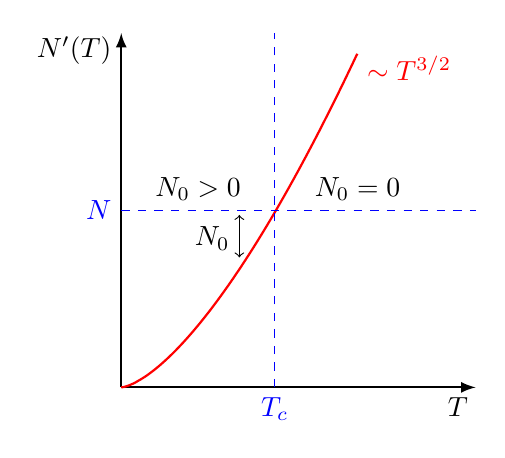
\begin{tikzpicture}[scale=1.5]
    \draw[thick, -latex] (0, 0) -- (0, 3);
    \draw[thick, -latex] (0, 0) -- (3, 0);
    \draw[red, thick, smooth, samples=100, domain=0:2] plot (\x, {\x^(3/2)});
    \node[red, right] at (2, 2.7) {$\sim T^{3/2}$};
    \node[below] at (2.85, 0) {$T$};
    \node[left] at (0, 2.85) {$N'(T)$};
    \draw[dashed, blue] (0, 1.5) -- (3, 1.5);
    \node[blue, left] at (0, 1.5) {$N$};
    \draw[dashed, blue] (1.3, 0) -- (1.3, 3);
    \node[below, blue] at (1.3, 0) {$T_c$};
    \draw[<->] (1, 1.46) -- (1, 1.1);
    \node[left] at (1, 1.26) {$N_0$};
    \node[above] at (0.65, 1.5) {$N_0 > 0$};
    \node[above] at (2, 1.5) {$N_0 = 0$};
\end{tikzpicture}
\end{document}